% This is a Basic Assignment Paper but with like Code and stuff allowed in it, there is also url, hyperlinks from contents included. 

\documentclass[11pt]{article}

% Preamble

\usepackage[margin=1in]{geometry}
\usepackage{amsfonts, amsmath, amssymb}
\usepackage{fancyhdr, float, graphicx}
\usepackage[utf8]{inputenc} % Required for inputting international characters
\usepackage[T1]{fontenc} % Output font encoding for international characters
\usepackage{fouriernc} % Use the New Century Schoolbook font
\usepackage[nottoc, notlot, notlof]{tocbibind}
\usepackage{listings}
\usepackage{xcolor}
\usepackage{blindtext}
\usepackage{hyperref}
\hypersetup{
    colorlinks=true,
    linkcolor=black,
    filecolor=magenta,      
    urlcolor=cyan,
    pdfpagemode=FullScreen,
    }

\definecolor{codegreen}{rgb}{0,0.6,0}
\definecolor{codegray}{rgb}{0.5,0.5,0.5}
\definecolor{codepurple}{rgb}{0.58,0,0.82}
\definecolor{backcolour}{rgb}{0.95,0.95,0.92}

\lstdefinestyle{mystyle}{
    backgroundcolor=\color{backcolour},   
    commentstyle=\color{codegreen},
    keywordstyle=\color{magenta},
    numberstyle=\tiny\color{codegray},
    stringstyle=\color{codepurple},
    basicstyle=\ttfamily\footnotesize,
    breakatwhitespace=false,         
    breaklines=true,                 
    captionpos=b,                    
    keepspaces=true,                 
    numbers=left,                    
    numbersep=5pt,                  
    showspaces=false,                
    showstringspaces=false,
    showtabs=false,                  
    tabsize=2
}

\lstset{style=mystyle}

% Header and Footer
\pagestyle{fancy}
\fancyhead{}
\fancyfoot{}
\fancyhead[L]{\textit{\Large{SET Assignment 3 - UML Diagrams}}}
%\fancyhead[R]{\textit{something}}
\fancyfoot[C]{\thepage}
\renewcommand{\footrulewidth}{1pt}



% Other Doc Editing
% \parindent 0ex
%\renewcommand{\baselinestretch}{1.5}

\begin{document}

\begin{titlepage}
	\centering

	%---------------------------NAMES-------------------------------

	\huge\textsc{
		MIT World Peace University
	}\\

	\vspace{0.75\baselineskip} % space after Uni Name

	\LARGE{
		Software Engineering and Testing\\
		Second Year B. Tech, Semester 4
	}

	\vfill % space after Sub Name

	%--------------------------TITLE-------------------------------

	\rule{\textwidth}{1.6pt}\vspace*{-\baselineskip}\vspace*{2pt}
	\rule{\textwidth}{0.6pt}
	\vspace{0.75\baselineskip} % Whitespace above the title



	\huge{\textsc{
			UML Use Case and Class Diagrams
		}} \\



	\vspace{0.5\baselineskip} % Whitespace below the title
	\rule{\textwidth}{0.6pt}\vspace*{-\baselineskip}\vspace*{2.8pt}
	\rule{\textwidth}{1.6pt}

	\vspace{1\baselineskip} % Whitespace after the title block

	%--------------------------SUBTITLE --------------------------	

	\LARGE\textsc{
		\centering
		Assignment No. 3 - \textit{UML Diagrams}\\
		and Assignment No. 4 - \textit{Class Diagrams}
	} % Subtitle or further description
	\vfill

	%--------------------------AUTHOR-------------------------------

	Prepared By
	\vspace{0.5\baselineskip} % Whitespace before the editors

	\Large{
		Krishnaraj Thadesar \\
		Cyber Security and Forensics\\
		Batch A1, PA 20
	}


	\vspace{0.5\baselineskip} % Whitespace below the editor list
	\today

\end{titlepage}


\tableofcontents
\thispagestyle{empty}
\clearpage

\setcounter{page}{1}

\section{Aim}
Object Oriented Analysis and design using UML diagrams: Draw Use case and Class
Diagram using Open-Source Tool.

\section{Objectives}

The tasks we have to do are:
\begin{enumerate}
	\item You will have to identify the main entities (objects) for this system.
	\item You will have to find out the relationships between these objects.
	\item You will have to find the necessary attributes and functions that need to be associated
	      with each object to implement the functionality mentioned above.
	\item You will make a final comprehensive diagram show and all objects and their relations
	      along with their attributes and functions.
\end{enumerate}

\section{Problem Statement}

\textbf{Draw UML Use Case Diagram and Class Diagram for The Following Problem:} \\

\textit{The Purpose of an Attandence Assistant App is to help reduce the time taken for recording the attendance of a classroom in a school or college. The app will be able to record the attendance of a class in a matter of a few Seconds with minimum Energy Expended. It will record data on cloud, and be accessible to all the Teachers.}\\

\section{Theory}

\subsection{Use Case Diagram}

\subsubsection{What is a Use Case Diagram}

\textit{A use case diagram is a graphical representation of the interactions between the elements of a system. It is a behavioral diagram that shows the functionality of a system using actors and use cases. Use cases are the actions that can be performed on the system to achieve a goal. Actors are the entities that interact with the system to perform these use cases. Use cases are represented as ovals and actors are represented as stick figures. A use case diagram is a dynamic diagram because it shows the behavior of the system.}

\subsubsection{What is the use of a Use Case Diagram}

\begin{enumerate}
	\item It is a graphical representation of the functional requirements of the system.
	\item It helps in understanding the system from the user's point of view.
	\item It is useful in understanding the functional requirements of the system.
	\item It helps in identifying the actors and use cases.
	\item It helps in identifying the relationships between actors and use cases.
	\item It helps in identifying the relationships between use cases.
\end{enumerate}

\subsubsection{Elements of a Use Case Diagram}

\begin{enumerate}
	\item \textbf{Use Case:} A use case is a set of actions that are performed by an actor to achieve a goal. It is a scenario that describes the interaction between a user and a system to achieve a particular goal. A use case is represented as an oval in a use case diagram.
	\item \textbf{Actor:} An actor is an entity that interacts with the system to perform a use case. An actor can be a person, an organization, a software system, or a device. An actor is represented as a stick figure in a use case diagram.
	\item \textbf{Relationships:} There are three types of relationships between actors and use cases.
	      \begin{enumerate}
		      \item \textbf{Association:} Association is a relationship between an actor and a use case. It shows that the actor is associated with the use case. It is represented as a line with a closed arrowhead. The arrowhead points from the actor to the use case.
		      \item \textbf{Generalization:} Generalization is a relationship between two use cases. It shows that one use case is a more general use case than the other use case. It is represented as a line with an open arrowhead. The arrowhead points from the more general use case to the more specific use case.
		      \item \textbf{Include:} Include is a relationship between two use cases. It shows that one use case is a part of the other use case. It is represented as a line with a solid arrowhead. The arrowhead points from the more general use case to the more specific use case.
		      \item \textbf{Extend:} Extend is a relationship between two use cases. It shows that one use case can be extended by the other use case. It is represented as a line with a dashed arrowhead. The arrowhead points from the more general use case to the more specific use case.
	      \end{enumerate}
\end{enumerate}


\begin{figure}[H]
	\centering
	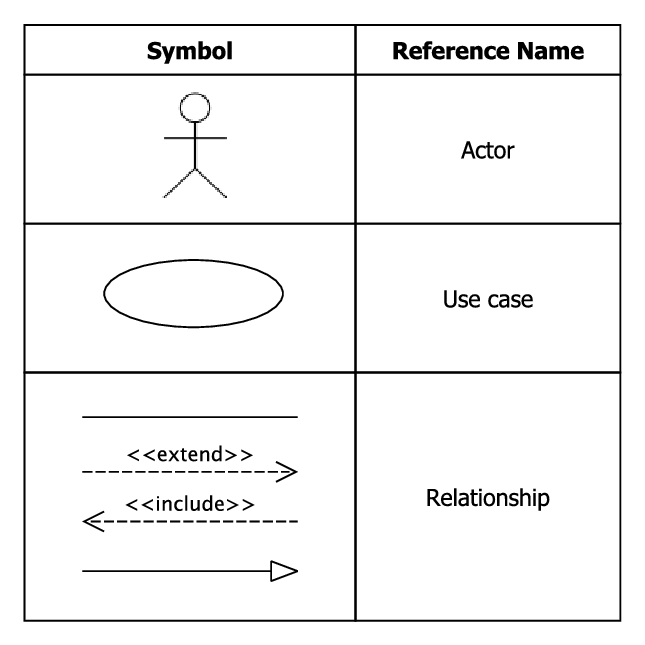
\includegraphics[scale=0.35]{Symbols-of-use-case-diagrams.png}
	\caption{Symbols of a Use Case Diagram}
\end{figure}

\clearpage

\subsection{Diagram}

\begin{figure}[H]
	\centering
	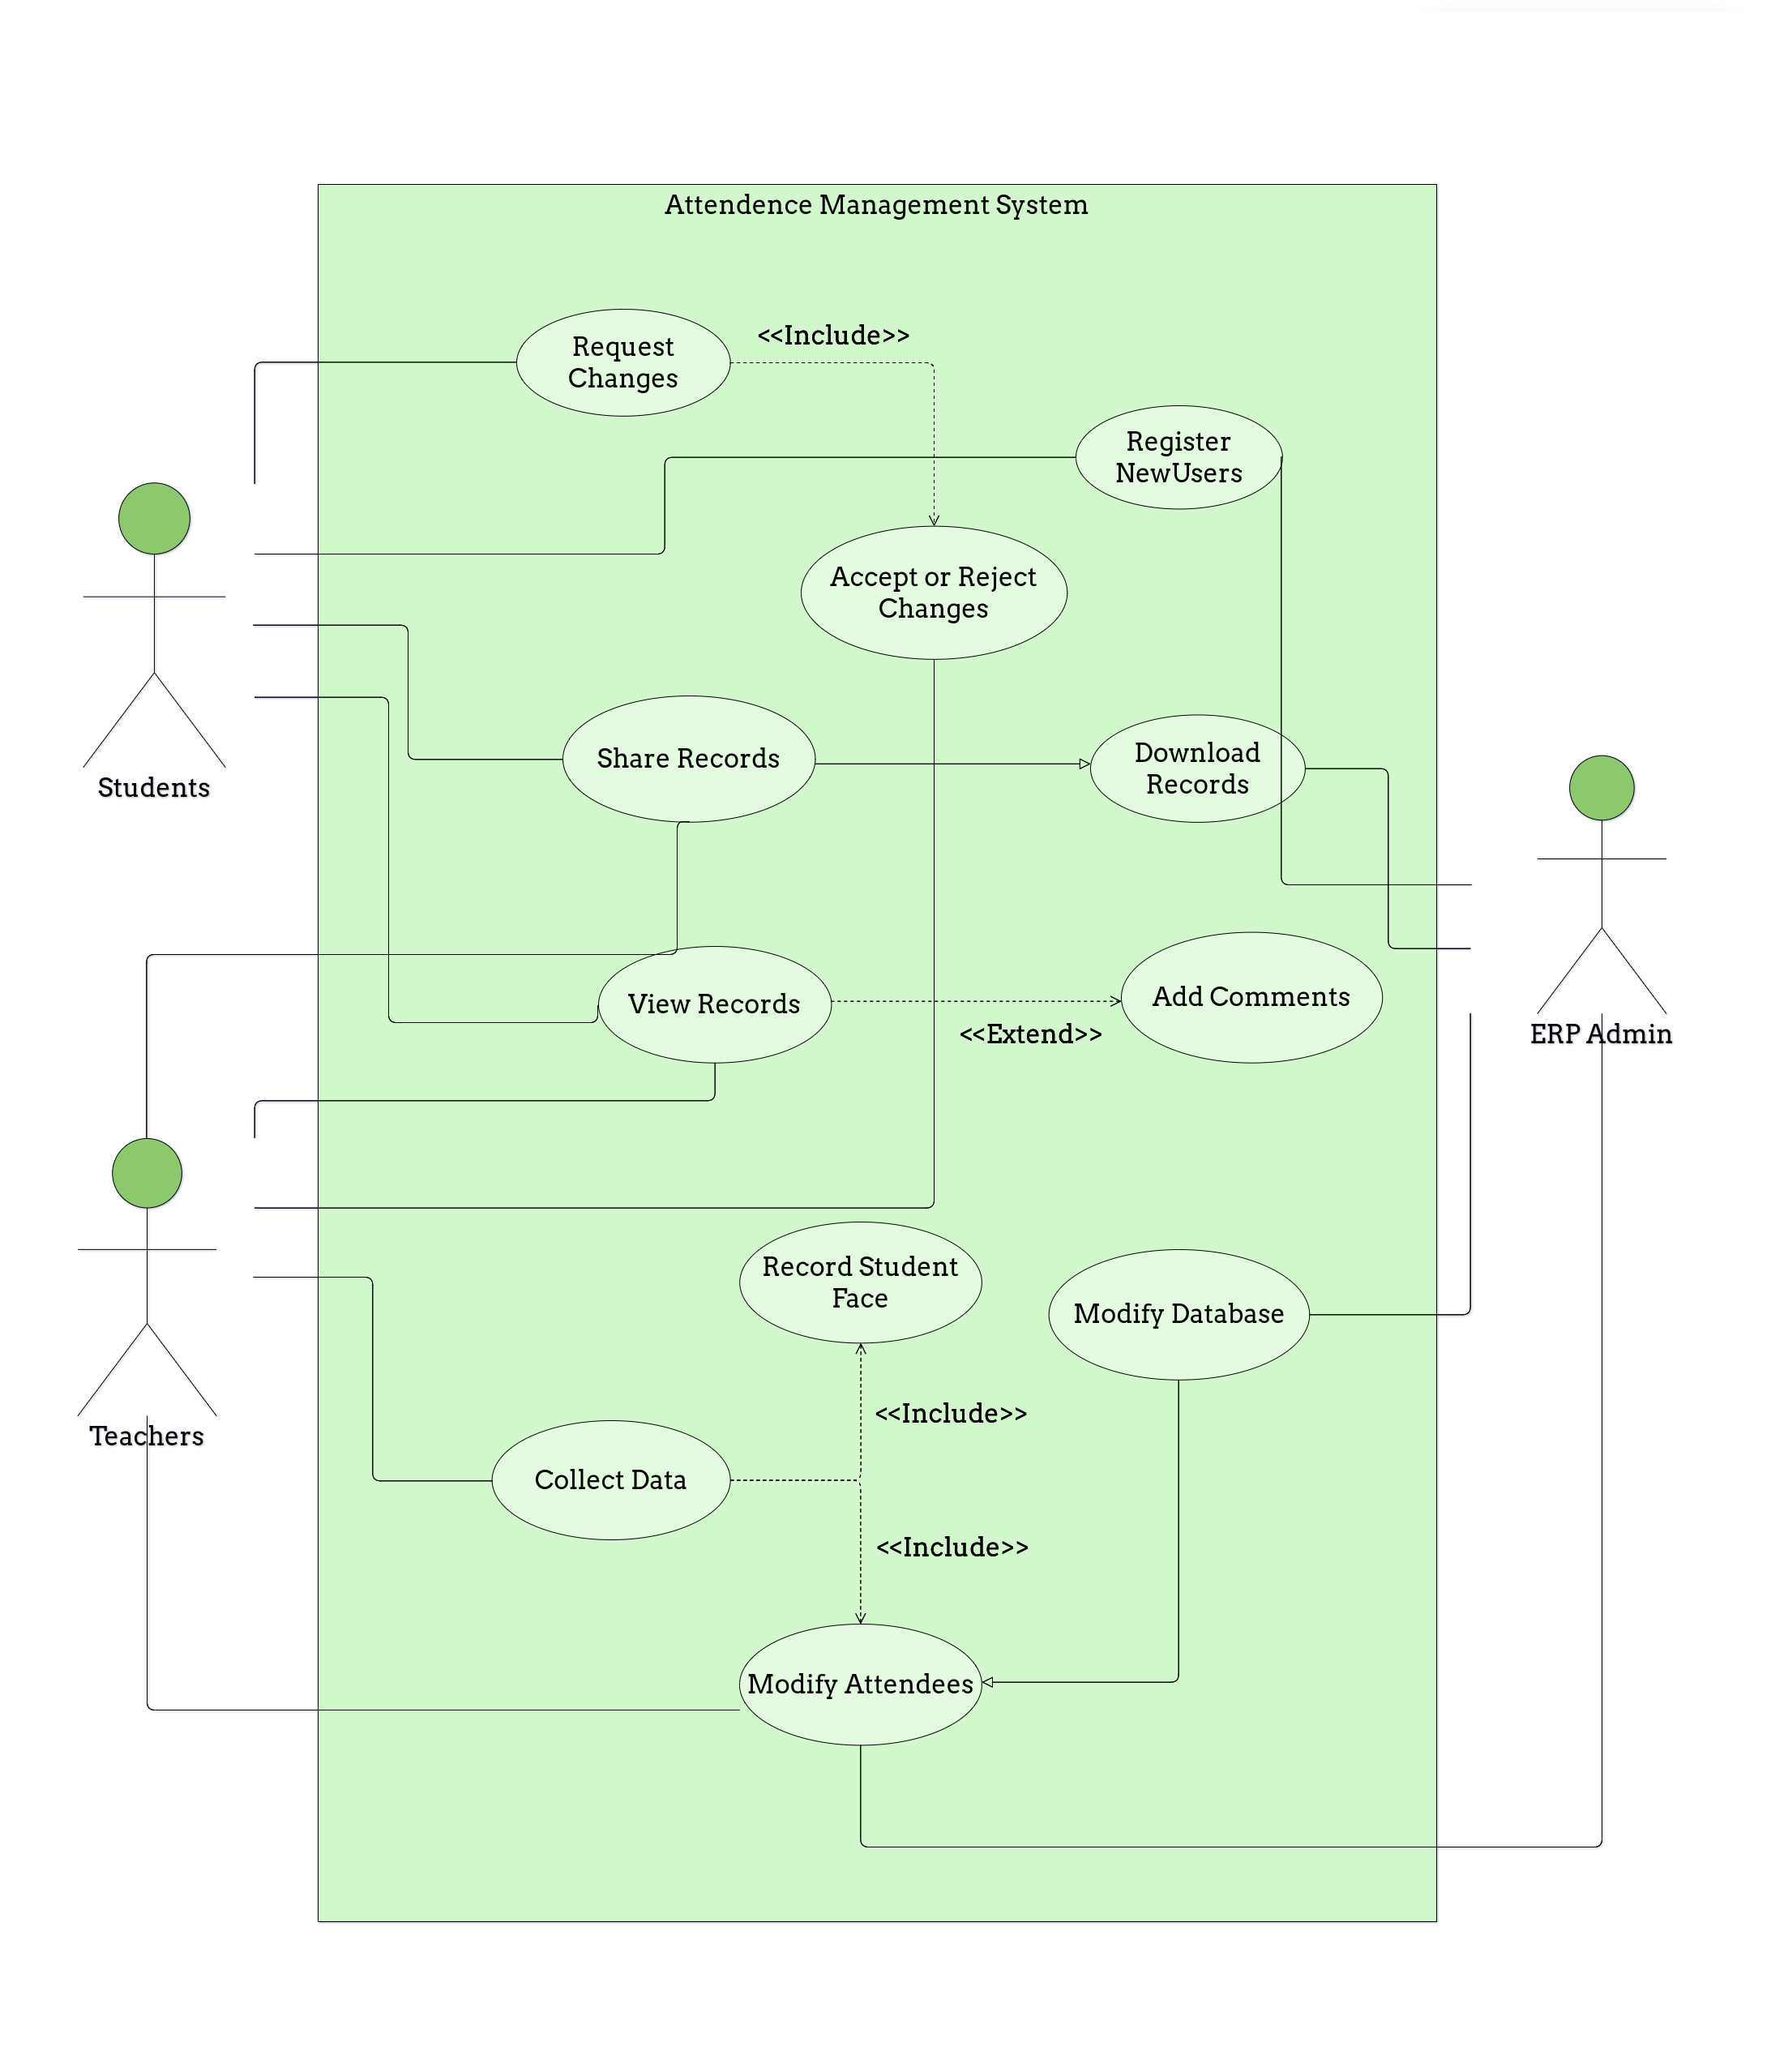
\includegraphics[scale=0.20]{use_case.png}
	\caption{Use Case Diagram}
\end{figure}

\subsection{Class Diagram}

\subsubsection{What is a Class Diagram}

\textit{A class diagram is a static diagram that shows the structure of a system. It is a structural diagram that shows the classes and their relationships in a system. It describes the attributes and operations of a class. It shows the static structure of a system.}

\subsubsection{What is the use of a Class Diagram}

\begin{enumerate}
	\item It is a graphical representation of the static structure of a system.
	\item It helps in understanding the structure of a system.
	\item It describes the classes and their relationships in a system.
	\item It describes the attributes and operations of a class.
	\item It is useful in identifying the classes of a system.
	\item It is useful in identifying the relationships between classes.
\end{enumerate}

\subsubsection{Elements of a Class Diagram}

\begin{enumerate}
	\item \textbf{Class:} A class is a collection of objects that have similar attributes and operations. It is the basic building block of object-oriented systems. A class is represented as a rectangle in a class diagram.
	\item \textbf{Attributes:} An attribute is a variable that describes the state of a class. It is a data member of a class. An attribute is represented as a variable in a class diagram.
	\item \textbf{Operations:} An operation is a behavior of a class. It is a function that describes the behavior of a class. An operation is represented as a function in a class diagram.
	\item \textbf{Relationships:} There are four types of relationships between classes.
	      \begin{enumerate}
		      \item \textbf{Association:} Association is a relationship between two classes. It shows that two classes are associated with each other. It is represented as a line with a closed arrowhead. The arrowhead points from the class that has a whole part relationship to the class that has a part-whole relationship.
		      \item \textbf{Generalization:} Generalization is a relationship between two classes. It shows that one class is a more general class than the other class. It is represented as a line with an open arrowhead. The arrowhead points from the more general class to the more specific class.
		      \item \textbf{Dependency:} Dependency is a relationship between two classes. It shows that one class is dependent on another class.
		      \item \textbf{Composition: } The composition is a special type of aggregation which denotes strong ownership between two classes when one class is a part of another class. For example, if college is composed of classes student. The college could contain many students, while each student belongs to only one college.
		      \item \textbf{Aggregation: } Aggregation. refers to the formation of a particular class as a result of one class being aggregated or built as a collection. For example, the class “library” is made up of one or more books, among other materials. In aggregation, the contained classes are not strongly dependent on the lifecycle of the container.
		      \item \textbf{Multiplicity: } Multiplicity can be set for attributes, operations, and associations in a UML class diagram, and for associations in a use case diagram. The multiplicity is an indication of how many objects may participate in the given relationship or the allowable number of instances of the element.
	      \end{enumerate}
\end{enumerate}

\begin{figure}[H]
	\centering
	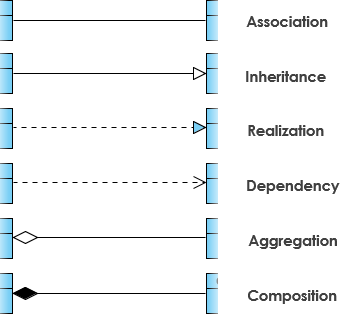
\includegraphics[scale=0.7]{07-relationships-between-classes.png}
	\caption{Relationships between Classes}
\end{figure}

\begin{figure}[H]
	\centering
	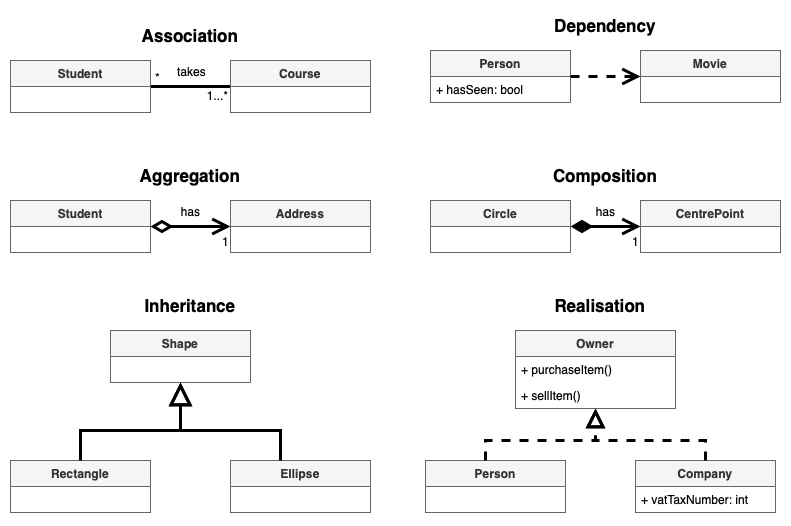
\includegraphics[scale=0.6]{uml-connectors.png}
	\caption{UML Connectors}
\end{figure}

\section{Procedure}

\subsection{Use Case Diagram}
\begin{enumerate}
	\item Create Actors to represent classes of people, organizations, other systems, software or
	      devices that interact with your system or subsystem.
	\item Create Use Cases for each of the goals that each actor seeks to achieve with the
	      system.
	\item Use Associations to link actors to use cases.
	\item Use <<include>> , <<extend>> and generalization to show the relationships among
	      the use cases
\end{enumerate}

\subsection{Class Diagram}
\begin{enumerate}
	\item Write a problem statement, clearly defining the scope of the system.
	\item List out nouns as the probable classes from the problem statement.
	\item Draw the classes of the nouns focus should be on understanding relationships.
	\item Draw model of the system- the class model. Show relationships, attributes and
	\item multiplicity in the class model. Data types not required.
\end{enumerate}

\subsection{Diagram}

% \begin{figure}[H]
% \centering
% \includegraphics[scale=0.5]{class_diagram.png}
% \caption{Class Diagram}
% \end{figure}

\section{Platform}
\textbf{Operating System}: Arch Linux x86-64 \\
\textbf{IDEs or Text Editors Used}: Visual Studio Code\\
\textbf{External Programs for Diagrams} : Draw.io\\


\section{Conclusion}
Thus, we learnt about Use case diagrams, and UML Class diagrams in detail.
\clearpage

\section{FAQ}


\begin{enumerate}
	\item \textbf{What kind of relationships do classes have? Explain all relationships with examples.}\\
	      \begin{enumerate}
		      \item \textbf{Association}: An association is a relationship between two classes, where one class uses an instance of the other class as a property or method parameter. Associations can be one-way or two-way. For example, in a library system, the "Book" class could be associated with the "Author" class because each book has one or more authors.

		      \item \textbf{Aggregation}: Aggregation is a type of association where one class is part of another class. The part class is typically a smaller part of the whole, and it can belong to more than one whole class. For example, a "Car" class can have a "Wheel" class, and each wheel can belong to many cars.

		      \item \textbf{Composition}: Composition is similar to aggregation, but the part class cannot exist outside the whole class. The whole class is responsible for creating and destroying its part classes. For example, a "House" class can have a "Room" class, and each room can only belong to one house.

		      \item \textbf{Inheritance}: Inheritance is a relationship where one class is a subclass of another class, inheriting its properties and methods. The subclass can add additional properties and methods or override the superclass's methods. For example, a "Student" class can inherit from a "Person" class, inheriting the properties of "name" and "age."

		      \item \textbf{Dependency}: Dependency is a relationship where one class depends on another class. If the dependent class changes, the class that depends on it may need to be modified. For example, a "Payment" class may depend on a "CreditCard" class, but if the credit card system changes, the payment class may need to be updated.
	      \end{enumerate}

	\item \textbf{Explain any 2 terminologies used in Use case diagrams.}\\

	      \begin{enumerate}
		      \item \textbf{Actors}: An actor is an external entity that interacts with the system. Actors are usually represented by stick figures in use case diagrams. Actors can be human users, other software systems, or even hardware devices. Actors are used to represent the roles that different users play in the system. For example, in a banking system, the "Customer" could be an actor who interacts with the system to perform tasks like depositing money, withdrawing money, and checking account balances.

		      \item \textbf{Use cases}: A use case is a set of actions or steps that a system performs to achieve a specific goal. Use cases describe the functionality of the system from a user's perspective. Each use case describes a specific task or process that the system can perform. Use cases are often represented as ovals in use case diagrams. For example, in a banking system, the "Withdraw Money" use case could describe the process that a customer follows to withdraw money from their account. The "Deposit Money" use case could describe the process that a customer follows to deposit money into their account.
	      \end{enumerate}

	\item \textbf{Explain the aggregation and composition in diagram?}\\

	      \begin{enumerate}
		      \item \textbf{Aggregation}: Aggregation is a "has-a" relationship between classes, where one class is made up of one or more instances of another class. In other words, a class contains a reference to another class, which can exist independently. In an aggregation relationship, the part class can belong to multiple whole classes at the same time.

		      \item \textbf{Composition}: Composition is a "part-of" relationship between classes, where one class is a part of another class. In other words, the part class cannot exist without the whole class, and a whole class can have only one instance of the part class. The part class's lifetime is controlled by the whole class, and if the whole class is destroyed, the part class is also destroyed.
	      \end{enumerate}

\end{enumerate}

\end{document}